% ==================================================
% Appendix: Analysis Statistics %
% ==================================================

\chapter[Analysis statistics]{Study of analysis statistics}
\label{appendix:statistics}

% Plan:
% Quantity of interest is the gaussian mean of the residual distribution in a region of interest.
% Typically, have 1 million triggers; for QS3.P.18 got 3.5 million triggers.
% See the drop off in peak residual mean error with more triggers (FIGURE).
% We are not statistically limited. Compare residual fits for L1 F34 between 1 million triggers and 3.5 million triggers: means don't change significantly.

Typically, one million triggers (cosmic muon events and noise) were collected for each Canadian quadruplet at McGill, resulting in roughly half the number of viable tracks after cuts in \package{tgc\_analysis/CosmicsAnalysis}. For QS3.P.18, 3.5 million triggers were collected. To gauge the sensitivity of the analysis to the available statistics, partitions of this data with each with a different number of triggers were analyzed separately. Ultimately, the quantity of interest was the gaussian mean of the residual distribution in regions of interest, so the peak in the distribution of the statistical uncertainty in the residuals means for each area of interest for a specific tracking combination was used to gauge the quality of the analysis. How the peak in the residual mean uncertainty distribution changes with the number of triggers is shown in figure \ref{fig:res_mean_uncert_vs_triggers}. 

\begin{figure}
    \centering
    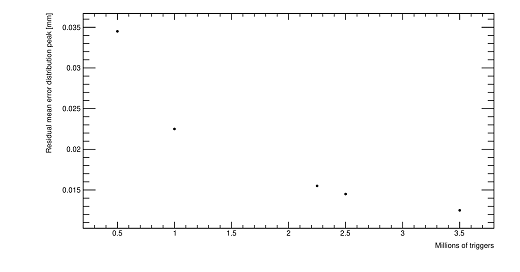
\includegraphics[width = \textwidth]{figures/figure_QS3P18_2900V_peakOfMeanErrorsDistVsTriggers_layer1_fixedlayers34_resize_33_percent.png}
    \caption{How the peak of the distributions of uncertainties in the residuals means in regions of interest for tracks on layer 1 built from hits on layers 3 and 4 changed with the number of triggers provided in the analysis. The distribution falls off as $~\frac{1}{\sqrt{N}}$ as expected.}
    \label{fig:res_mean_uncert_vs_triggers}
\end{figure}

The distribution falls off as roughly  